\chapter{Vyhodnocení}\label{chapter-results}

V~této kapitole popisujeme v~sekci~\ref{methods} způsob vyhodnocení našeho systému,
v~sekci~\ref{results} výsledky tohoto vyhodnocení a v~sekci~\ref{improvements}
vylepšení, která jsme na základě výsledků navrhli, spolu s~nápady k~jejich implementaci.

\section{Způsob vyhodnocení}\label{methods}

Běžné způsoby vyhodnocování dialogových systémů popisují
\citet[sekce 24.5]{jurafsky_slp_2020}, podrobněji pak ještě \citet{Deriu_2020}.
U~systémů zaměřených na plnění úkolů je primárním měřítkem poměr úspěšných
splnění cíle. U~jiných druhů úkolů než je náš, kde je potřeba vyplnit více slotů, je možné
sledovat ještě podrobněji poměr správně vyplněných slotů. Náš systém však
vyplňuje pouze jméno, tedy řešit poměr splněných úkolů je dostatečné.

Vytvořili jsme dotazník, v~jehož úvodu jsme popsali náš systém a způsob instalace
aplikace, a následně se uživatelů dotazovali především na počet pokusů o~hovor a
množství úspěšných zahájení hovoru. Dále nás zajímalo, jak často (na stupnici
nikdy -- málokdy -- občas -- často -- vždy) se objevily
tyto problémy:
\begin{itemize}
    \item chyba při inicializaci,
    \item špatně rozpoznaný hlas,
    \item jméno nerozpoznáno WA,
    \item jméno nenalezeno v~kontaktech, i když mělo být,
    \item ke jménu nalezeny neodpovídající kontakty,
    \item nalezeno více kontaktů a výběr z~nich se nepodařil,
    \item hlas byl rozpoznán, ale nepřišla žádná odpověď,
    \item celá aplikace selhala.
\end{itemize}
Následující otázky se týkaly návrhů na opravy a vylepšení, dále jsme zjišťovali celkový
zájem o~podobnou aplikaci. Z~důvodu kontroly implementace jsme přidali ještě
dotaz na verzi systému, který uživatel měl ve svém mobilním telefonu při testování. Dotazník je
možné najít v~příloze~\ref{appendix-quest}.

\section{Výsledky}\label{results}

Grafy úspěšnosti a popularity ukazuje obrázek~\ref{img-charts},
frekventovanost konkrétnějších problémů pak tabulka~\ref{tab-results}.

\paragraph{Celková úspěšnost} Podařilo se nám získat \(15\) testovacích uživatelů, kteří dohromady uskutečnili 91
pokusů o~hovor, z~toho \(51\) bylo úspěšných, jak znázorňuje
graf na obrázku~\ref{img-ratio-succ}. Celková úspěšnost
systému tedy byla \(56\,\rm \%\), ale s~relativně velkým rozptylem. U~některých uživatelů
byly úspěšné skoro všechny pokusy, u~některých skoro žádné. Z~analýzy záznamů ve WA usuzujeme,
že rozdíl dělá především způsob komunikace a jména uložených kontaktů daného
uživatele.

\paragraph{Popularita} Zájem o~podobnou aplikaci ukazuje graf na obrázku~\ref{img-ratio-interest}.
Pouze 3 z~15 uživatelů uvedli, že by o~takovou aplikaci neměli vůbec zájem.
Zbylí by o~takovou aplikaci měli zájem, pokud by fungovala lépe, přidala nové funkce,
případně oboje.

% \begin{figure}[h]
%     \centering
%     \subfloat[Graf úspěšnosti splnění úkolu.]%
%     {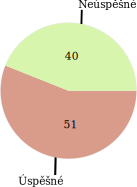
\includegraphics[width=0.28\textwidth]{../img/chart-succ.pdf}}
%     \hfill%
%     \subfloat[Graf zájmu o podobnou aplikaci.]%
%     {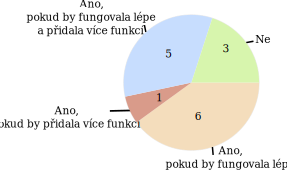
\includegraphics[width=0.6\textwidth]{../img/chart-interest.pdf}}
% \end{figure}

\newsavebox{\tempbox}
\begin{figure}[H]
    \sbox{\tempbox}{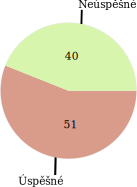
\includegraphics[width=0.28\textwidth]{../img/chart-succ.pdf}}
    \subfloat[Úspěšnost plnění.]{\usebox{\tempbox}\label{img-ratio-succ}}%
    \qquad
    \subfloat[Zájem o~podobnou aplikaci.]{\vbox to \ht\tempbox{%
            \vfil
            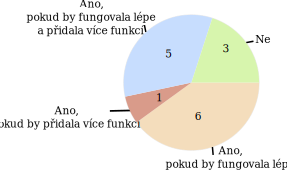
\includegraphics[width=0.6\textwidth]{../img/chart-interest.pdf}
            \vfil}\label{img-ratio-interest}}%
    \caption{Grafy výsledků.}\label{img-charts}
\end{figure}

\begin{table}[b!]

    \centering
    %%% Tabulka používá následující balíčky:
    %%%   - booktabs (\toprule, \midrule, \bottomrule)
    %%%   - dcolumn (typ sloupce D: vycentrovaná čísla zarovnaná na
    %%%     desetinnou čárku
    %%%     Všimněte si, že ve zdrojovém kódu jsou desetinné tečky, ale
    %%%     tisknou se čárky.
    %%% Dále používáme příkazy \pulrad a \mc definované v makra.tex

    \begin{tabular}{l@{\hspace{1.5cm}}D{.}{,}{3.2}D{.}{,}{1.2}D{.}{,}{2.3}D{.}{,}{2.3}D{.}{,}{2.3}}
        \toprule
        \textbf{Problém}        & \mc{Nikdy} & \mc{Málokdy} & \mc{Občas} & \mc{Často} & \mc{Vždy} \\
        \midrule
        Inicializace            & 10         & 4            & 1          & 0          & 0         \\
        Bez odpovědi            & 11         & 3            & 1          & 0          & 0         \\
        Celkové selhání         & 11         & 3            & 1          & 0          & 0         \\
        Rozpoznávání řeči       & 8          & 2            & 4          & 1          & 0         \\
        Detekce entity WA       & 7          & 4            & 1          & 3          & 0         \\
        Nenalezení kontaktů     & 7          & 3            & 1          & 3          & 1         \\
        Neodpovídající kontakty & 9          & 2            & 2          & 1          & 1         \\
        Výběr z~kontaktů        & 6          & 1            & 5          & 1          & 2         \\
        \bottomrule
        \multicolumn{6}{l}{}
    \end{tabular}

    \caption{Počty uživatelů, kteří uvedli danou frekventovanost daného problému.}\label{tab-results}

\end{table}

\paragraph{Inicializace} Co se týká konkrétnějších nedostatků, u~otázek na inicializaci, rozpoznání
hlasu bez odpovědi a celkové selhání všichni až na jednoho uživatele odpověděli,
že toto byl problém nikdy nebo málokdy. U~inicializace za příčinu
chyby považujeme nenainstalované či zakázané Google TTS, v~rámci
implementace by asi bylo vhodné toto kontrolovat.

\paragraph{Rozpoznávání řeči} Špatně rozpoznaný hlas uvedlo jako problém občas nebo často 5 z~15 uživatelů.
To je nezanedbatelné množství, avšak protože používáme STT službu
třetí strany, nemůžeme diskutovat o~příčině.

\paragraph{Detekce entity WA a nenalezení kontaktů} Podobně častými problémy bylo nerozpoznání
jména ve WA a nenalezení kontaktů k~zadanému vstupu. Oba
tyto problémy označil 1 uživatel jako občasné, 3 jako časté, nenalezení kontaktu
navíc 1 uživatel jako komplikaci vždy.

\paragraph{Neodpovídající kontakty} Frekventovaným problémem bylo nalezení neodpovídajících kontaktů,
což u\-ve\-dl 1 uživatel jako vždy, 1 jako často a 2 jako občas.

\paragraph{Výběr z~kontaktů} Největším problémem bylo nalezení více kontaktů a nezdařený výběr z~nich.
2 uživatelé uvedli, že to byl problém vždy, 1 že často a 5 že
občas. Zde viníme především nedostatky porovnávací komponenty, kontroluje
totiž čistě odpovídající části kontaktu a vstupu. V~případě, že uživatel
řekne \uv{Jan Novák} a má uloženy kontakty \uv{Jan Novák} a \uv{Jan Novák starší},
komponenta oběma přiřadí plnou jistotu a nedokáže mezi nimi vybrat.

\paragraph{Žádané opravy} Nutnou opravou je z~pohledu uživatelů lepší rozpoznávání jmen i přiřazování
kontaktů k~nim, za důležité také zmínili potvrzení vytáčení ještě jedním
\uv{ano/ne}. Několikrát byla zmíněna také plynulost aplikace a rychlost
odpovědi.

\paragraph{Žádaná vylepšení} Nejvíce žádaným vylepšením byla schopnost rozpoznávat libovolný název kontaktu
místo čistě jmen, mnoho uživatelů využívá názvy kontaktů \uv{Mamka} a podobné.
Několikrát zmíněným vítaným vylepšením by také byla schopnost posílat textové
zprávy.

\section{Vylepšení a jejich možná implementace}\label{improvements}

V~této sekci se budeme zabývat nutnými a možnými vylepšeními, která
vyplynula z~vyhodnocení s~uživateli. V~podsekci~\ref{better-match}
uvedeme návrhy na zlepšení porovnávání uživatelova vstupu s~jeho
seznamem kontaktů. V~podsekci~\ref{better-app} pak navrhneme
úpravy v~aplikaci, které by vedly k~lepšímu uživatelskému
zážitku, pokud by cílem bylo čistě vytáčení kontaktů.

\subsection{Zkvalitnění přiřazování}\label{better-match}

Největším problémem bylo přiřazování názvů kontaktů spolu s~neschopností přiřadit
názvy, které nejsou českými jmény. Z~hlediska implementačního se o~tuto část
stará WA, naše porovnávací komponenta pracuje až s~entitami rozpoznanými jím.
Jako možná řešení vidíme rozšířit základnu entit, se kterými WA pracuje. Ke
každému jménu bychom mohli získat domácké formy (jako \uv{Honza} ke jménu \uv{Jan})
a přidat je do WA, kromě nich ještě běžné názvy rodinných příslušníků,
které uživatelé často využívají jako názvy kontaktů (\uv{Mamka}, \uv{Babička}).
Pro zpřesnění bychom mohli přidat i relevantní vyskloňované tvary jmen (ke jménu \uv{Jan}
také \uv{Janu}, \uv{Janovi}, \uv{Jana}).

Další možností by bylo snažit se v~této omezené doméně hledat jmenné entity na
základě vzorců. Když uživatel říká \uv{zavolej}, obvykle následuje název
kontaktu.

Poslední možností je přepracovat porovnávací komponentu, aby nebyla závislá
na entitách rozpoznaných pomocí WA. Touto cestou se pravděpodobně vydáme,
protože nám dává největší volnost implementace a především velkou
použitelnost mimo konkrétní doménu.

Jistě nutným vylepšením porovnávací komponenty je také přidání závislosti
limitu vzdálenosti na délce slov, které porovnáváme. V~aktuální verzi
totiž využíváme stejný limit 3 pro všechna slova, jak jsme popsali
v~podsekci~\ref{subsection-matching}. To u~krátkých slov umožní
přiřazení i kompletně rozdílných slov, zatímco u~dlouhých
slov je tento limit v~kombinaci s~komplikovaným skloňováním češtiny
příliš malý.

Dále pak vyřešení problému popsaného v~sekci~\ref{results}, totiž zohlednění
toho, že nějaký kontakt odpovídá naprosto
přesně a jiný obsahuje v~názvu další slova.

\subsection{Přepracování mobilní aplikace}\label{better-app}

Většina uživatelů uvedla, že by o~aplikaci měla zájem, pakliže by fungovala
lépe. Pokud bychom se zaměřili čistě na vytáčení kontaktů, obešli bychom se
bez celé detekce úmyslů a mohli celý dialog velmi zjednodušit.
Navrhovaný běh by pak vypadal následovně (podrobněji popisujeme dále):
\begin{code}
    Uživatel: /Stiskne tlačítko/
    Systém:   /Začne naslouchat/
    Uživatel: Název Kontaktu
    Systém:   /Porovnává celý vstup s kontakty přímo v zařízení/
    Systém:   Chcete zavolat Název Kontaktu?
    Uživatel: Ano
    Systém:   /Zahájí hovor/
\end{code}
Uživatel by stiskem
tlačítka zapnul rozpoznávání řeči a řekl jen název kontaktu,
kterému chce zavolat. Celý tento vstup by byl přímo v~zařízení
porovnán se všemi jmény kontaktů v~seznamu, pravděpodobně za
využití knihovny \texttt{JavaWuzzy}.\footnote{\url{https://github.com/xdrop/fuzzywuzzy}} Pokud by byl
nalezen jeden ostře lépe odpovídající kontakt, aplikace
by oznámila úmysl mu volat a uživatel by potvrdil \uv{ano/ne}.
Pokud by odpovídalo více kontaktů, ale méně než 4, uživatel
by z~nich dostal na výběr. Pokud by jich bylo více, dostal by
žádost o~zpřesnění požadavku. Celou dobu by bylo možné slovem
\uv{znovu} či obdobným začít od začátku.

Tím, že by celé řízení dialogu i porovnání mohlo probíhat v~aplikaci,
dosáhli bychom větší plynulosti aplikace, neboť bychom nemuseli čekat
na vyřízení síťových požadavků. Zjednodušením by se celý dialog také
výrazně zrychlil, což je žádoucí, protože zahájení hovoru by mělo
být rychlé.

Ideální variantou by pak bylo, kdyby i rozpoznání a generování řeči
dokázalo běžet lokálně v~aplikaci bez nutnosti kontaktování serveru.
Celá aplikace by pak mohla běžet offline. Zde by mohl pomoci projekt
\texttt{DeepSpeech}.\footnote{\url{https://github.com/mozilla/DeepSpeech}}
Pro trénink rozpoznání by bylo možné využít data, která prezentují \citet{kratochvil-etal-2020-large}.
Vhodná trénovací data pro syntézu řeči se nám najít nepodařilo. Vytvořením
otevřených datasetů v~mnoha jazycích se zabývá projekt Common Voice \citep{commonvoice_2020},
kam může kdokoliv dobrovolně přispět.